%%
%% This is file `sample-sigconf.tex',
%% generated with the docstrip utility.
%%
%% The original source files were:
%%
%% samples.dtx  (with options: `sigconf')
%% 
%% IMPORTANT NOTICE:
%% 
%% For the copyright see the source file.
%% 
%% Any modified versions of this file must be renamed
%% with new filenames distinct from sample-sigconf.tex.
%% 
%% For distribution of the original source see the terms
%% for copying and modification in the file samples.dtx.
%% 
%% This generated file may be distributed as long as the
%% original source files, as listed above, are part of the
%% same distribution. (The sources need not necessarily be
%% in the same archive or directory.)
%%
%% The first command in your LaTeX source must be the \documentclass command.
\documentclass[sigconf]{acmart}

\usepackage{listings}

%%
%% \BibTeX command to typeset BibTeX logo in the docs
\AtBeginDocument{%
  \providecommand\BibTeX{{%
    \normalfont B\kern-0.5em{\scshape i\kern-0.25em b}\kern-0.8em\TeX}}}

%% Rights management information.  This information is sent to you
%% when you complete the rights form.  These commands have SAMPLE
%% values in them; it is your responsibility as an author to replace
%% the commands and values with those provided to you when you
%% complete the rights form.
%\setcopyright{acmcopyright}
%\copyrightyear{2018}
%\acmYear{2018}
%\acmDOI{10.1145/1122445.1122456}

%% These commands are for a PROCEEDINGS abstract or paper.
%\acmConference[Woodstock '18]{Woodstock '18: ACM Symposium on Neural
%  Gaze Detection}{June 03--05, 2018}{Woodstock, NY}
%\acmBooktitle{Woodstock '18: ACM Symposium on Neural Gaze Detection,
%  June 03--05, 2018, Woodstock, NY}
%\acmPrice{15.00}
%\acmISBN{978-1-4503-9999-9/18/06}


%%
%% Submission ID.
%% Use this when submitting an article to a sponsored event. You'll
%% receive a unique submission ID from the organizers
%% of the event, and this ID should be used as the parameter to this command.
%%\acmSubmissionID{123-A56-BU3}

%%
%% The majority of ACM publications use numbered citations and
%% references.  The command \citestyle{authoryear} switches to the
%% "author year" style.
%%
%% If you are preparing content for an event
%% sponsored by ACM SIGGRAPH, you must use the "author year" style of
%% citations and references.
%% Uncommenting
%% the next command will enable that style.
%%\citestyle{acmauthoryear}

%%
%% end of the preamble, start of the body of the document source.
\begin{document}

%%
%% The "title" command has an optional parameter,
%% allowing the author to define a "short title" to be used in page headers.
\title{NaturalSelection: A Python package for user-friendly evolution of neural networks}

%%
%% The "author" command and its associated commands are used to define
%% the authors and their affiliations.
%% Of note is the shared affiliation of the first two authors, and the
%% "authornote" and "authornotemark" commands
%% used to denote shared contribution to the research.
\author{Dan Saattrup Nielsen}
\email{dan.nielsen@bristol.ac.uk}
\affiliation{%
  \institution{University of Bristol}
  \country{United Kingdom}
}

%%
%% By default, the full list of authors will be used in the page
%% headers. Often, this list is too long, and will overlap
%% other information printed in the page headers. This command allows
%% the author to define a more concise list
%% of authors' names for this purpose.

%%
%% The abstract is a short summary of the work to be presented in the
%% article.
\begin{abstract}
  Hyperparameter optimisation of neural networks is an incredibly time consuming process. A grid search is usually too time consuming, and a random search does base its search on prior results and is therefore still wasteful. Other approaches include Bayesian optimisation and genetic algorithms, both of which are ``guided'', meaning that they base the choice of hyperparameters on past performance. We propose a new Python package, NaturalSelection, which provides a simple Pythonic API for applying genetic algorithms to general optimisation problems, with built-in support for tuning both the hyperparameters and architecture of neural networks. Several other Python packages that optimise hyperparameters of neural networks exist, but these are utilising algorithms that tune the hyperparameters not including the architecture, such as learning rate, momentum and batch size. Our package ``evolves'' a neural network, starting from a shallow network and gradually making it more complex while optimising performance. As a side benefit this prioritises simpler neural architectures, resulting in faster training times.
\end{abstract}

%%
%% The code below is generated by the tool at http://dl.acm.org/ccs.cfm.
%% Please copy and paste the code instead of the example below.
%%

%%
%% Keywords. The author(s) should pick words that accurately describe
%% the work being presented. Separate the keywords with commas.
\keywords{Neural networks, hyperparameter optimization, hyperparameter tuning, genetic algorithm, python}

%%
%% This command processes the author and affiliation and title
%% information and builds the first part of the formatted document.
\maketitle

\section{Example}

Here is an example of finding a multilayer perceptron to model the well-known dataset Fashion-MNIST. Here the \textsf{fashion\_mnist\_train\_val\_sets} function fetches the dataset and performs standard normalisation preprocessing.

\lstset{caption = Evolution of a population of MLPs}
\begin{lstlisting}
  >>> import naturalselection as ns
  >>> nns = ns.NNs(
  ...   size = 20,
  ...   train_val_sets = train_val_sets(),
  ...   loss_fn = 'categorical_crossentropy',
  ...   score = 'accuracy',
  ...   output_activation = 'softmax',
  ...   max_epochs = 1,
  ...   max_training_time = 120,
  ...   )
  ...
  >>> history = nns.evolve(generations = 20)
  Evolving population: 100%|===| 20/20 [1:32:00<00:00]
  Computing fitness: 100%|=======| 11/11 [05:37<00:00]
  >>> 
  >>> history.fittest
  {'genome': {'optimizer': 'adamax', 
  'activation': 'relu', 'batch_size': 32, 
  'initializer': 'glorot_uniform', 
  'input_dropout': 0.0, 
  'neurons0': 256, 'dropout0': 0.3, 
  'neurons1': 512, 'dropout1': 0.3,
  'neurons2': 128, 'dropout2': 0.0, 
  'neurons3': 0, 'dropout3': 0.1,
  'neurons4': 1024, 'dropout4': 0.2}, 
  'fitness': 0.855400025844574}
\end{lstlisting}

From the evolved population we can then plot the evolution.
\lstset{caption = Plotting the evolution}
\begin{lstlisting}
  >>> history.plot(
  ...   title = "Validation accuracy by generation",
  ...   ylabel = "Validation accuracy"
  ...   )
\end{lstlisting}

\begin{center}
  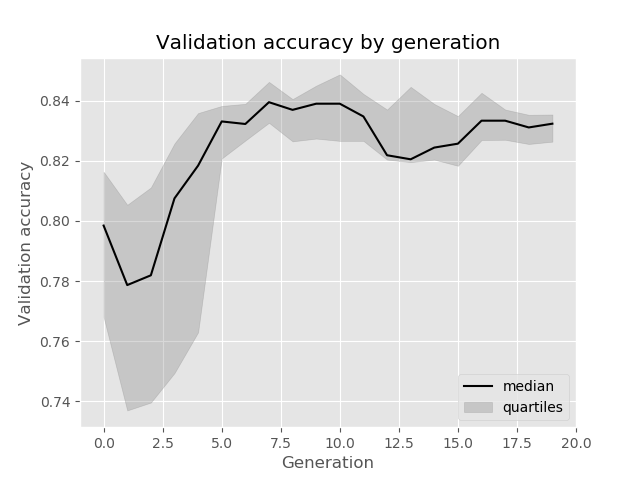
\includegraphics[scale=0.42]{gfx/fashion_mnist_example.png}
\end{center}

Lastly, we can train the best performing model and save it locally:

\lstset{caption = Saving the optimised model}
\begin{lstlisting}
  >>> # Training the best model and saving 
  >>> # it to fashion_mnist_model.h5
  >>> best_score = nns.train_best(
  ...   file_name = 'fashion_mnist_model'
  ...   )
  Epoch 0: 100%|====| 60000/60000 [00:21<00:00]
  (...)
  Epoch 44: 100%|===| 60000/60000 [00:21<00:00]
  >>>
  >>> best_score
  0.9029
\end{lstlisting}

\end{document}
\endinput
%%
%% End of file `sample-sigconf.tex'.
